% Lines starting with a percent sign (%) are comments. LaTeX will 
% not process those lines. Similarly, everything after a percent 
% sign in a line is considered a comment. To produce a percent sign
% in the output, write \% (backslash followed by the percent sign). 
% ==================================================================
% Usage instructions:
% ------------------------------------------------------------------
% The file is heavily commented so that you know what the various
% commands do. Feel free to remove any comments you don't need from
% your own copy. When redistributing the example thesis file, please
% retain all the comments for the benefit of other thesis writers! 
% ==================================================================
% Compilation instructions: 
% ------------------------------------------------------------------
% Use pdflatex to compile! Input images are expected as PDF files.
% Example compilation:
% ------------------------------------------------------------------
% > pdflatex thesis-example.tex
% > bibtex thesis-example
% > pdflatex thesis-example.tex
% > pdflatex thesis-example.tex
% ------------------------------------------------------------------
% You need to run pdflatex multiple times so that all the cross-references
% are fixed. pdflatex will tell you if you need to re-run it (a warning
% will be issued)  
% ------------------------------------------------------------------
% Compilation has been tested to work in ukk.cs.hut.fi and kosh.hut.fi
% - if you have problems of missing .sty -files, then the local LaTeX
% environment does not have all the required packages installed.
% For example, when compiling in vipunen.hut.fi, you get an error that
% tikz.sty is missing - in this case you must either compile somewhere
% else, or you cannot use TikZ graphics in your thesis and must therefore
% remove or comment out the tikz package and all the tikz definitions. 
% ------------------------------------------------------------------

% General information
% ==================================================================
% Package documentation:
% 
% The comments often refer to package documentation. (Almost) all LaTeX
% packages have documentation accompanying them, so you can read the
% package documentation for further information. When a package 'xxx' is
% installed to your local LaTeX environment (the document compiles
% when you have \usepackage{xxx} and LaTeX does not complain), you can 
% find the documentation somewhere in the local LaTeX texmf directory
% hierarchy. In ukk.cs.hut.fi, this is /usr/texlive/2008/texmf-dist,
% and the documentation for the titlesec package (for example) can be 
% found at /usr/texlive/2008/texmf-dist/doc/latex/titlesec/titlesec.pdf.
% Most often the documentation is located as a PDF file in 
% /usr/texlive/2008/texmf-dist/doc/latex/xxx, where xxx is the package name; 
% however, documentation for TikZ is in
% /usr/texlive/2008/texmf-dist/doc/latex/generic/pgf/pgfmanual.pdf
% (this is because TikZ is a front-end for PGF, which is meant to be a 
% generic portable graphics format for LaTeX).
% You can try to look for the package manual using the ``find'' shell
% command in Linux machines; the find databases are up-to-date at least
% in ukk.cs.hut.fi. Just type ``find xxx'', where xxx is the package
% name, and you should find a documentation file.
% Note that in some packages, the documentation is in the DVI file
% format. In this case, you can copy the DVI file to your home directory,
% and convert it to PDF with the dvipdfm command (or you can read the
% DVI file directly with a DVI viewer).
% 
% If you can't find the documentation for a package, just try Googling
% for ``latex packagename''; most often you can get a direct link to the
% package manual in PDF format.
% ------------------------------------------------------------------


% Document class for the thesis is report
% ------------------------------------------------------------------
% You can change this but do so at your own risk - it may break other things.
% Note that the option pdftext is used for pdflatex; there is no
% pdflatex option. 
% ------------------------------------------------------------------
\documentclass[12pt,a4paper,oneside,pdftex]{report}

% The input files (tex files) are encoded with the latin-1 encoding 
% (ISO-8859-1 works). Change the latin1-option if you use UTF8 
% (at some point LaTeX did not work with UTF8, but I'm not sure
% what the current situation is) 
\usepackage[latin1]{inputenc}
% OT1 font encoding seems to work better than T1. Check the rendered
% PDF file to see if the fonts are encoded properly as vectors (instead
% of rendered bitmaps). You can do this by zooming very close to any letter 
% - if the letter is shown pixelated, you should change this setting 
% (try commenting out the entire line, for example).  
\usepackage[OT1]{fontenc}
% The babel package provides hyphenating instructions for LaTeX. Give
% the languages you wish to use in your thesis as options to the babel
% package (as shown below). You can remove any language you are not
% going to use.
% Examples of valid language codes: english (or USenglish), british, 
% finnish, swedish; and so on.
\usepackage[finnish,english]{babel}


% Font selection
% ------------------------------------------------------------------
% The default LaTeX font is a very good font for rendering your 
% thesis. It is a very professional font, which will always be 
% accepted. 
% If you, however, wish to spicen up your thesis, you can try out
% these font variants by uncommenting one of the following lines
% (or by finding another font package). The fonts shown here are 
% all fonts that you could use in your thesis (not too silly). 
% Changing the font causes the layouts to shift a bit; you many
% need to manually adjust some layouts. Check the warning messages
% LaTeX gives you.
% ------------------------------------------------------------------
% To find another font, check out the font catalogue from
% http://www.tug.dk/FontCatalogue/mathfonts.html
% This link points to the list of fonts that support maths, but
% that's a fairly important point for master's theses.
% ------------------------------------------------------------------
% <rant>
% Remember, there is no excuse to use Comic Sans, ever, in any
% situation! (Well, maybe in speech bubbles in comics, but there 
% are better options for those too)
% </rant>

% \usepackage{palatino}
% \usepackage{tgpagella}



% Optional packages
% ------------------------------------------------------------------
% Select those packages that you need for your thesis. You may delete
% or comment the rest.

% Natbib allows you to select the format of the bibliography references.
% The first example uses numbered citations: 
\usepackage[square,sort&compress,numbers]{natbib}
% The second example uses author-year citations.
% If you use author-year citations, change the bibliography style (below); 
% acm style does not work with author-year citations.
% Also, you should use \citet (cite in text) when you wish to refer
% to the author directly (\citet{blaablaa} said blaa blaa), and 
% \citep when you wish to refer similarly than with numbered citations
% (It has been said that blaa blaa~\citep{blaablaa}).
% \usepackage[square]{natbib}

% The alltt package provides an all-teletype environment that acts
% like verbatim but you can use LaTeX commands in it. Uncomment if 
% you want to use this environment. 
% \usepackage{alltt}

% The eurosym package provides a euro symbol. Use with \euro{}
\usepackage{eurosym} 

% Verbatim provides a standard teletype environment that renderes
% the text exactly as written in the tex file. Useful for code
% snippets (although you can also use the listings package to get
% automatic code formatting). 
\usepackage{verbatim}

% The listing package provides automatic code formatting utilities
% so that you can copy-paste code examples and have them rendered
% nicely. See the package documentation for details.
% \usepackage{listings}

% The fancuvrb package provides fancier verbatim environments 
% (you can, for example, put borders around the verbatim text area
% and so on). See package for details.
% \usepackage{fancyvrb}

% Supertabular provides a tabular environment that can span multiple 
% pages. 
%\usepackage{supertabular}
% Longtable provides a tabular environment that can span multiple 
% pages. This is used in the example acronyms file. 
\usepackage{longtable}

% The fancyhdr package allows you to set your the page headers 
% manually, and allows you to add separator lines and so on. 
% Check the package documentation. 
% \usepackage{fancyhdr}

% Subfigure package allows you to use subfigures (i.e. many subfigures
% within one figure environment). These can have different labels and
% they are numbered automatically. Check the package documentation. 
%\usepackage{subfigure}
\usepackage{subcaption}
% The titlesec package can be used to alter the look of the titles 
% of sections, chapters, and so on. This example uses the ``medium'' 
% package option which sets the titles to a medium size, making them
% a bit smaller than what is the default. You can fine-tune the 
% title fonts and sizes by using the package options. See the package
% documentation.
\usepackage[medium]{titlesec}

% The TikZ package allows you to create professional technical figures.
% The learning curve is quite steep, but it is definitely worth it if 
% you wish to have really good-looking technical figures. 
\usepackage{tikz}
% You also need to specify which TikZ libraries you use
\usetikzlibrary{positioning}
\usetikzlibrary{calc}
\usetikzlibrary{arrows}
\usetikzlibrary{decorations.pathmorphing,decorations.markings}
\usetikzlibrary{shapes}
\usetikzlibrary{patterns}



\usepackage{caption}
% The aalto-thesis package provides typesetting instructions for the
% standard master's thesis parts (abstracts, front page, and so on)
% Load this package second-to-last, just before the hyperref package.
% Options that you can use: 
%   mydraft - renders the thesis in draft mode. 
%             Do not use for the final version. 
%   doublenumbering - [optional] number the first pages of the thesis
%                     with roman numerals (i, ii, iii, ...); and start
%                     arabic numbering (1, 2, 3, ...) only on the 
%                     first page of the first chapter
%   twoinstructors  - changes the title of instructors to plural form
%   twosupervisors  - changes the title of supervisors to plural form
\usepackage[mydraft,twosupervisors]{aalto-thesis}
%\usepackage[mydraft,doublenumbering]{aalto-thesis}
%\usepackage{aalto-thesis}


% Hyperref
% ------------------------------------------------------------------
% Hyperref creates links from URLs, for references, and creates a
% TOC in the PDF file.
% This package must be the last one you include, because it has
% compatibility issues with many other packages and it fixes
% those issues when it is loaded.   
\RequirePackage[pdftex]{hyperref}
% Setup hyperref so that links are clickable but do not look 
% different
\hypersetup{colorlinks=false,raiselinks=false,breaklinks=true}
\hypersetup{pdfborder={0 0 0}}
\hypersetup{bookmarksnumbered=true}
% The following line suggests the PDF reader that it should show the 
% first level of bookmarks opened in the hierarchical bookmark view. 
\hypersetup{bookmarksopen=true,bookmarksopenlevel=1}
% Hyperref can also set up the PDF metadata fields. These are
% set a bit later on, after the thesis setup.   


% Thesis setup
% ==================================================================
% Change these to fit your own thesis.
% \COMMAND always refers to the English version;
% \FCOMMAND refers to the Finnish version; and
% \SCOMMAND refers to the Swedish version.
% You may comment/remove those language variants that you do not use
% (but then you must not include the abstracts for that language)
% ------------------------------------------------------------------
% If you do not find the command for a text that is shown in the cover page or
% in the abstract texts, check the aalto-thesis.sty file and locate the text
% from there. 
% All the texts are configured in language-specific blocks (lots of commands
% that look like this: \renewcommand{\ATCITY}{Espoo}.
% You can just fix the texts there. Just remember to check all the language
% variants you use (they are all there in the same place). 
% ------------------------------------------------------------------
\newcommand{\TITLE}{OpenEM Performance Characteristics in Realtime Stream Processing on a Multicore DSP}
\newcommand{\FTITLE}{OpenEM:n Suorituskykyominaisuudet Reaaliaikaisessa Virtalaskennassa Moniydin DSP:ll�}
\newcommand{\SUBTITLE}{}
\newcommand{\FSUBTITLE}{}
\newcommand{\SSUBTITLE}{}
\newcommand{\DATE}{June 18, 2011}
\newcommand{\FDATE}{18. kes�kuuta 2011}
\newcommand{\SDATE}{Den 18 Juni 2011}

% Supervisors and instructors
% ------------------------------------------------------------------
% If you have two supervisors, write both names here, separate them with a 
% double-backslash (see below for an example)
% Also remember to add the package option ``twosupervisors'' or
% ``twoinstructors'' to the aalto-thesis package so that the titles are in
% plural.
% Example of one supervisor:
%\newcommand{\SUPERVISOR}{Professor Antti Yl�-J��ski}
%\newcommand{\FSUPERVISOR}{Professori Antti Yl�-J��ski}
%\newcommand{\SSUPERVISOR}{Professor Antti Yl�-J��ski}
% Example of twosupervisors:
\newcommand{\SUPERVISOR}{Professor Antti Yl�-J��ski\\
  Professor Pekka Perustieteilij�}
\newcommand{\FSUPERVISOR}{Professori Antti Yl�-J��ski\\
  Professori Pekka Perustieteilij�}
\newcommand{\SSUPERVISOR}{Professor Antti Yl�-J��ski\\
  Professor Pekka Perustieteilij�}

% If you have only one instructor, just write one name here
\newcommand{\INSTRUCTOR}{Olli Ohjaaja M.Sc. (Tech.)}
\newcommand{\FINSTRUCTOR}{Diplomi-insin��ri Olli Ohjaaja}
\newcommand{\SINSTRUCTOR}{Diplomingenj�r Olli Ohjaaja}
% If you have two instructors, separate them with \\ to create linefeeds
% \newcommand{\INSTRUCTOR}{Olli Ohjaaja M.Sc. (Tech.)\\
%  Elli Opas M.Sc. (Tech)}
%\newcommand{\FINSTRUCTOR}{Diplomi-insin��ri Olli Ohjaaja\\
%  Diplomi-insin��ri Elli Opas}
%\newcommand{\SINSTRUCTOR}{Diplomingenj�r Olli Ohjaaja\\
%  Diplomingenj�r Elli Opas}

% If you have two supervisors, it is common to write the schools
% of the supervisors in the cover page. If the following command is defined,
% then the supervisor names shown here are printed in the cover page. Otherwise,
% the supervisor names defined above are used.
\newcommand{\COVERSUPERVISOR}{Professor Antti Yl�-J��ski, Aalto University\\
  Professor Pekka Perustieteilij�, University of Helsinki}

% The same option is for the instructors, if you have multiple instructors.
% \newcommand{\COVERINSTRUCTOR}{Olli Ohjaaja M.Sc. (Tech.), Aalto University\\
%  Elli Opas M.Sc. (Tech), Aalto SCI}


% Other stuff
% ------------------------------------------------------------------
\newcommand{\PROFESSORSHIP}{}
\newcommand{\FPROFESSORSHIP}{}
\newcommand{\SPROFESSORSHIP}{}
% Professorship code is the same in all languages
\newcommand{\PROFCODE}{T-110}
\newcommand{\KEYWORDS}{}
\newcommand{\FKEYWORDS}{}
\newcommand{\SKEYWORDS}{}
\newcommand{\LANGUAGE}{English}
\newcommand{\FLANGUAGE}{Englanti}
\newcommand{\SLANGUAGE}{Engelska}

% Author is the same for all languages
\newcommand{\AUTHOR}{Risto Vuorio}


% Currently the English versions are used for the PDF file metadata
% Set the PDF title
\hypersetup{pdftitle={\TITLE\ \SUBTITLE}}
% Set the PDF author
\hypersetup{pdfauthor={\AUTHOR}}
% Set the PDF keywords
\hypersetup{pdfkeywords={\KEYWORDS}}
% Set the PDF subject
\hypersetup{pdfsubject={Master's Thesis}}


% Layout settings
% ------------------------------------------------------------------

% When you write in English, you should use the standard LaTeX 
% paragraph formatting: paragraphs are indented, and there is no 
% space between paragraphs.
% When writing in Finnish, we often use no indentation in the
% beginning of the paragraph, and there is some space between the 
% paragraphs. 

% If you write your thesis Finnish, uncomment these lines; if 
% you write in English, leave these lines commented! 
% \setlength{\parindent}{0pt}
% \setlength{\parskip}{1ex}

% Use this to control how much space there is between each line of text.
% 1 is normal (no extra space), 1.3 is about one-half more space, and
% 1.6 is about double line spacing.  
% \linespread{1} % This is the default
% \linespread{1.3}

% Bibliography style
% acm style gives you a basic reference style. It works only with numbered
% references.
\bibliographystyle{acm}
% Plainnat is a plain style that works with both numbered and name citations.
% \bibliographystyle{plainnat}


% Extra hyphenation settings
% ------------------------------------------------------------------
% You can list here all the files that are not hyphenated correctly.
% You can provide many \hyphenation commands and/or separate each word
% with a space inside a single command. Put hyphens in the places where
% a word can be hyphenated.
% Note that (by default) LaTeX will not hyphenate words that already
% have a hyphen in them (for example, if you write ``structure-modification 
% operation'', the word structure-modification will never be hyphenated).
% You need a special package to hyphenate those words.
\hyphenation{di-gi-taa-li-sta yksi-suun-tai-sta}



% The preamble ends here, and the document begins. 
% Place all formatting commands and such before this line.
% ------------------------------------------------------------------
\begin{document}
% This command adds a PDF bookmark to the cover page. You may leave
% it out if you don't like it...
\pdfbookmark[0]{Cover page}{bookmark.0.cover}
% This command is defined in aalto-thesis.sty. It controls the page 
% numbering based on whether the doublenumbering option is specified
\startcoverpage

% Cover page
% ------------------------------------------------------------------
% Options: finnish, english, and swedish
% These control in which language the cover-page information is shown
\coverpage{english}


% Abstracts
% ------------------------------------------------------------------
% Include an abstract in the language that the thesis is written in,
% and if your native language is Finnish or Swedish, one in that language.

% Abstract in English
% ------------------------------------------------------------------
\thesisabstract{english}{}

% Abstract in Finnish
% ------------------------------------------------------------------
\thesisabstract{finnish}{}

% Acknowledgements
% ------------------------------------------------------------------
% Select the language you use in your acknowledgements
\selectlanguage{english}

% Uncomment this line if you wish acknoledgements to appear in the 
% table of contents
%\addcontentsline{toc}{chapter}{Acknowledgements}

% The star means that the chapter isn't numbered and does not 
% show up in the TOC
\chapter*{Acknowledgements}
\vskip 10mm

\noindent Espoo, \DATE
\vskip 5mm
\noindent\AUTHOR

% Acronyms
% ------------------------------------------------------------------
% Use \cleardoublepage so that IF two-sided printing is used 
% (which is not often for masters theses), then the pages will still
% start correctly on the right-hand side.
\cleardoublepage
% Example acronyms are placed in a separate file, acronyms.tex
\addcontentsline{toc}{chapter}{Abbreviations and Acronyms}
\chapter*{Abbreviations and Acronyms}

% The longtable environment should break the table properly to multiple pages,
% if needed

\noindent
\begin{longtable}{@{}p{0.25\textwidth}p{0.7\textwidth}@{}}
    4CIF & 4 x CIF \\
    API & Application Programming Interface \\
    CCS & Code Composer Studio \\
    CIF & Common Intermediate Format \\
    CPU & Central Processing Unit \\
    DDF & Dynamic Dataflow \\
    DDR & Double Data Rate \\
    DMA & Direct Memory Access \\
    DPDK & Dataplane Development Kit \\
    DSP & Digital Signal Processor \\
    EMIF & External Memory Interface \\
    EO & Execution Object \\
    FLOPS & Floating-point Operations Per Second \\
    FPGA & Field-Programmable Gate Array \\
    GPU & Graphics Processing Unit \\
    IDE & Integrated Development Environment \\
    L1 & Level 1 cache \\
    L2 & Level 2 cache \\
    MCSDK & Multicore Software Development Kit \\
    MPEG & Moving Picture Experts Group \\
    MSM & Multicore Shared Memory \\
    MSMC & Multicore Shared Memory Controller \\
    MoC & Model of Computation \\
    NSN & Nokia Solutions and Networks \\
    NTSC & National Television System Committee \\
    OpenEM & Open Event Machine \\
    PCI & Peripheral Component Interconnect \\
    PDSP & Packed Data Structure Processor \\
    PKTDMA & Packet Direct Memory Access \\
    PiSDF & Parameterized and Interfaced Synchronous Dataflow \\
    QCIF & Quarter CIF \\
    RGB & Red Green Blue \\
    S-LAM & System-Level Architecture Model \\
    SDF & Synchronous Dataflow \\
    SoC & System on a Chip \\
    TI & Texas Instruments \\
    UI & User Interface \\
    YCbCr & YCbCr color space \\
    YUV & YUV color space \\
\end{longtable}


% Table of contents
% ------------------------------------------------------------------
\cleardoublepage
% This command adds a PDF bookmark that links to the contents.
% You can use \addcontentsline{} as well, but that also adds contents
% entry to the table of contents, which is kind of redundant.
% The text ``Contents'' is shown in the PDF bookmark. 
\pdfbookmark[0]{Contents}{bookmark.0.contents}
\tableofcontents

% List of tables
% ------------------------------------------------------------------
% You only need a list of tables for your thesis if you have very 
% many tables. If you do, uncomment the following two lines.
% \cleardoublepage
% \listoftables

% Table of figures
% ------------------------------------------------------------------
% You only need a list of figures for your thesis if you have very 
% many figures. If you do, uncomment the following two lines.
% \cleardoublepage
% \listoffigures

% The following label is used for counting the prelude pages
\label{pages-prelude}
\cleardoublepage

%%%%%%%%%%%%%%%%% The main content starts here %%%%%%%%%%%%%%%%%%%%%
% ------------------------------------------------------------------
% This command is defined in aalto-thesis.sty. It controls the page 
% numbering based on whether the doublenumbering option is specified
\startfirstchapter

% Add headings to pages (the chapter title is shown)
\pagestyle{headings}

% The contents of the thesis are separated to their own files.
% Edit the content in these files, rename them as necessary.
% ------------------------------------------------------------------
\chapter{Introduction}
\label{chapter:intro}

\section{Problem statement}

\section{Structure of the Thesis}
\label{section:structure} 


Potentially confusing concepts are explained here. The background section in the thesis will be written to explain the context to a reader who's not familiar with the problem space. The background chapter will explain 1. How the thesis fits in to context of Industrial Internet. 2. Why stream processing is an important problem. 3. What kinds of programming models are used. 4. Why DSPs are a promising candidate for stream processing. 5. ... 

\textbf{Stream Processing} is a programming paradigm that aims to simplify the design of parallel programs. In stream processing computations happen in kernel functions. The kernel functions are applied upon each element of the input stream. Stream Processing is a high level programming model and can be implemented in a multitude of ways. Stream Processing is called uniform if all data is processed by all kernels. (NVIDIA Streaming Multiprocessor references this type of streaming.) \\http://en.wikipedia.org/wiki/Stream\_processing

\textbf{Stream Computing} is often considered in IoT or Industrial Internet context. In Stream Computing data is not in the memory as in V. Neumann architecture but in a ``stream'' that passes through the process. A problem or a task involving lots of continuous I/O without necessarily knowing the end of the input is a stream computing problem.

\textbf{Flow}, a high-level concept where computations happen when dependencies are updates. For example excel implements kind of flow computation.

\textbf{Dataflow Programming} models a program as a directed graph of data flowing between operations. Operations have explicitly defined inputs and outputs. Operations are carried out as soon as the inputs to that particular operation become valid. The explicit dependencies between the operations make Dataflow Programming well suited for parallel processing because when the operation becomes ready it can be executed any time on any hardware resource without further need for considering its dependencies.\\http://en.wikipedia.org/wiki/Dataflow\_programming

\textbf{Dataflow Architecture} is a hardware architecture in which the execution of instructions is based on the availability of input arguments. The execution order of the instructions is thus indeterministic.\\http://en.wikipedia.org/wiki/Dataflow\_architecture

\textbf{Dataflow (computing)} is a software architecture based on the Flow concept. Writing software in dataflow pattern helps reduce coupling related code in programs, meaning programmers need to write less code to explicitly update values based on their dependencies.\\http://en.wikipedia.org/wiki/Dataflow\\http://en.wikipedia.org/wiki/Kahn\_process\_networks

\textbf{Actor model} Actors can be thought of as similar to OOP objects but with special emphasis on parallelism. Anything actors do can be done in parallel with other actors. In actor model all computations are done in actors. Actor model is based on the idea of actors sending messages to each other. As a response to receiving a message an actor can create more actors, send messages, change how to respond to next message etc. Actors can send messages at any time, but the receiver can respond whenever it is ready.\\http://en.wikipedia.org/wiki/Actor\_model
This section describes the hardware platform used in the experiments. The experiments were conducted on a Texas Instruments TMS320C6678 multi-core digital signal processor. First, the selection of the TMS320C6678 as the hardware platform for the experiments in this thesis is explained in subsection~\ref{subsec:selection-of-platform}. Second, an overview of the hardware platform is given in subsection~\ref{subsec:hw-overview}. After the overview, the key features of the platform are described in subsections \ref{subsec:c66x} C66x DSP, \ref{subsec:c66memory} Memory Hierarchy and \ref{subsec:multicorenav} Multicore Navigator.

\subsection{Selection of the Hardware Platform}
\label{subsec:selection-of-platform}
This thesis investigates stream processing with Open Event Machine on a multi-core DSP. The Texas Instruments Keystone I family of multi-core DSPs has an advanced support for multi-core programming, including a Texas Instruments implementation of OpenEM~\cite{MCSDKbrochure}. The multi-core programming support has not always been a design priority of multi-core DSPs, for example the TMS320C647x DSPs were looked at as, "multiple single-core DSP in a single package" by the programmers~\cite{openemwhite}.

The hardware platform used in the experiments in this thesis is the Texas Instrument TMS320C6678. The TMS320C6678 is a fixed and floating point digital signal processor based on the Texas Instruments Keystone I architecture~\cite{tmsdatasheet}. The Keystone I architecture was selected because there exists an OpenEM implementation for that supports the processors implementing the architecture. Out of the Keystone I devices TMS320C6678 was selected because Advantech provides an evaluation module TMDXEVM6678L for the specific processor, which makes the experimentation more straightforward than building an evaluation platform from scratch. Another benefit of the TMS320C6678 is that the PREESM rapid prototyping tool for dataflow applications has support for it~\cite{pelcat2014preesm}.

\subsection{TMS320C6678 Overview}
\label{subsec:hw-overview}

\begin{figure}[h!]
    \begin{center}
        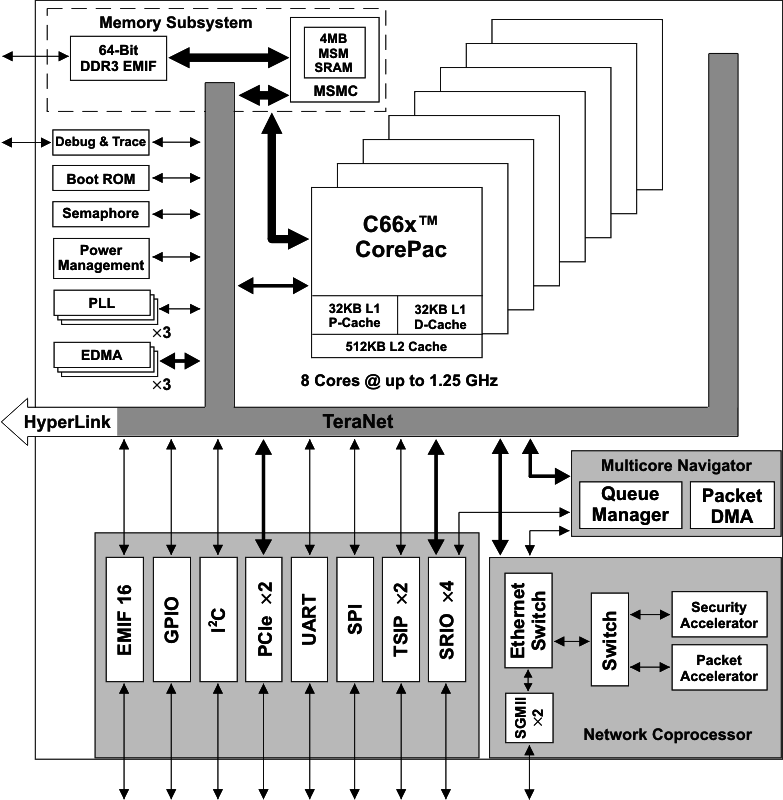
\includegraphics[width=0.99\textwidth]{images/fbd_SPRS691e.png}
        \caption{High-level schematic of the TMS320C6678 architecture. Figure from~\cite{tmsdatasheet}.}
        \label{fig:arch_overview}
    \end{center}
\end{figure}

The TMS320C6678 is based on the Keystone I architecture. The Keystone I architecture specifies a set of hardware elements which enable integration of C66x DSP cores, application specific co-processors and IO \cite{tmsdatasheet}. The Keystone I hardware modules and their connections are presented in the figure \ref{fig:arch_overview}. The points of interest in the figure in the scope of this thesis are the C66x CorePac cores depicted in the middle of the figure, the memory subsystems and its components in the top-left of the figure and the Multicore Navigator depicted in the right edge of the figure.

In the Keystone I architecture there are multiple ways for the C66x cores to communicate with each other, the memory and the peripherals. The methods of communication of specific interest for the experiments in this thesis are communication through shared memory discussed in subsection \ref{subsec:c66memory} and communication through packet based communication manager Multicore Navigator introduced in subsection \ref{subsec:multicorenav}.

The development board used for development of the experiment applications and measurements is an Advantech TMDXEVM6678L. TMDXEVM6678L is an evaluation module for the TMS320C6678 multi-core DSP. The evaluation module has 512 megabytes of DDR3 memory which is sufficient for stream processing applications. Another important feature of the evaluation module is the emulator module with USB connectivity. The emulator together with the Code Composer Studio IDE (CCS) make the programming and debugging the experiment programs for the DSPs uncomplicated.~\cite{evmref} CCS version 5.2 is distributed with the hardware evaluation module and was used for development of the experiments in this thesis.

\subsection{C66x DSP}
\label{subsec:c66x}
The hardware platform used in this thesis is the TMS320C6678. The TMS320C6678 consists of eight C66x DSP cores. The C66x is based on the Texas Instruments TMS320C66x instruction set architecture. The TMS320C66x is a very long instruction word architecture, which allows for high amount of instruction level parallelism. The C66x has a total of eight functional units, which operate in parallel. This means that the C66x can dispatch up to eight instructions per cycle. The instructions dispatched in parallel move through pipeline stages simultaneously. Pipelining helps eliminate CPU stalls while waiting for memory operations or other CPU instructions taking multiple cycles complete.~\cite{sprugh7}

Keeping the utilization of the wide pipeline high, the CPU needs to have enough registers to prevent excessive memory access stalling. The CPU has 64 32-bit general purpose registers~\cite{sprugh7}. The C66x is a high-end processor with native support for 32-bit and 64-bit floating point instructions and capability of clock speeds up to 1.4 GHz~\cite{sprugh7}.

\subsection{Memory Hierarchy}
\label{subsec:c66memory}
The TMS320C6678 contains a multi-layer memory hierarchy which can be configured by the user to a large extent. The memory hierarchy in the device consists of L1 and L2 memories for each core, Multicore Shared Memory (MSM) and additionally external memory provided by the evaluation module. In the figure~\ref{fig:arch_overview} the memories are placed inside the subsystems they are part of, MSM can be found in the upper-left corner as part of the memory subsystem.

Each c66x CPU has 32 KB level 1 program cache (L1P), 32 KB level 1 data cache (L1D). Each CPU also has 512 KB of level 2 cache. Both of the L1 caches and the L2 cache can be found in the figure~\ref{fig:arch_overview} as part of the C66x CorePac box. Initially after bootup both L1P and L1D are configured as cache but they can be reconfigured as addressable memory by software. The L2 memory is always configured as addressable memory after reset but can be configured as cache by software. \cite{tmsdatasheet} L2 SRAM addresses are always cached with L1P and L1D whereas external memory addresses are configured noncacheable by default~\cite{cacheguide}.

Configuring the state of the L1 and L2 memories as well as other memory configurations can be handled with software \cite{sprugh7}. CCS automatically handles a lot of the memory mapping needed for applications and provides tools for creating custom configurations.

In PC hardware cache coherence is usually handled automatically by the hardware. In c66x, however, that is not the case. Each c66x core maintains cache coherence between its L1 caches and the L2 cache automatically but programmer needs to manage coherence in most other cases. For example if caching is enabled for an external memory region shared by two cores, explicit cache coherence operations need to be performed before each core can read from or write to the shared region~\cite{cacheguide}.

The evaluation module has 512 MB of DDR3 memory \cite{evmref}. The memory in the evaluation module, as any external memory in other hardware configurations, is accessible through the Multicore Shared Memory Controller (MSMC). The MSMC itself contains 4096KB of shared memory accesible by all cores. In the figure~\ref{fig:arch_overview} the memory subsystem contains the EMIF link to the external memory and the MSMC.

\subsection{Multicore Navigator}
\label{subsec:multicorenav}
The multi-core programmability of the TMS320C6678 makes it interesting for this thesis. The device is designed to allow simple co-operation of the DSP cores and provides the required hardware support for that purpose. The core features enabling the multi-core programmability are grouped under the name of Multicore Navigator.

Multicore Navigator is the name for a collection of features in Keystone I and II devices, which enables hardware-accelerated, packet-based communication between on-chip devices. Texas Instruments claims the use of specialized hardware for on-chip communication results in significant performance gains when implemented carefully. The design goals stated for the Multicore Navigator in \cite{navigator} are minimizing host interaction and maximizing memory use efficiency.~\cite{navigator}

In Keystone I devices such as the TMS320C6678, the Multicore Navigator provides a hardware queue manager, a special direct memory access for different subsystems called Packet DMA (PKTDMA), and multi-core host notifications via interrupts. \cite{navigator} The Texas Instruments OpenEM implementation \ref{chapter:openem} heavily utilizes the features provided by Multicore Navigator.

The Queue Manager on Keystone I architecture devices is a hardware module that manages 8192 queues. Packets are queued and dequeued from the queues by the applications. The Queue Manager is responsible for accelerating the packet communication. In addition to the Queue Manager the Queue Management Subsystem contains two Packed Data Structure Processors (PSDP) which perform tasks related to the queue management and packet communication. For example the PDSP processors can be used to perform accumulation of packets. The accumulation program is given a list of queues to poll. Whenever it finds a descriptor from one of the queues it is watching it will pop the descriptor and place it in a buffer provided by the application. After a pre-determined number of descriptors, or after reaching its time limit, the accumulator program notifies the host processor about the descriptors in the buffer via an interrupt. Use of such firmware offloads the burden of queue polling from the host processors.~\cite{navigator} The TI implementation of OpenEM \ref{chapter:openem} provides its own firmware for the PDSP cores which is utilized by the OpenEM runtime for event scheduling \cite{openemwhite}.

The PKTDMA is a special DMA utilized by the Multicore Navigator to transfer packet buffers between memory locations. When a packet is sent to a queue The PKTDMA reads the address of the data to be transferred from packet descriptor, transfers the data in one or more data moves and writes the pointer to the data queue specified as the receiver of the packet. The PKTDMA is useful because it allows the program running on a PDSP core to move data in the memory without interrupting the host processors.~\cite{navigator} OpenEM uses PKTDMA to move event buffers to the caches of the core, which is about to receive the event~\cite{openemwhite}.

\chapter{Open Event Machine}
\label{chapter:openem}
This thesis investigates the suitability of Open Event Machine (OpenEM) for
real-time stream processing. OpenEM is a programming framework for event-driven
multicore applications.

\section{OpenEM Framework}
\subsection{Overview}
OpenEM is an event-driven programming framework originally developed for the
networking data plane by Nokia Solutions and Networks. The OpenEM framework
provides a programming model for scalable and dynamically load balanced
applications. The key components of the OpenEM programming model are events,
execution objects, queues and the scheduler. OpenEM works with
run-to-completion principle which means once an event begins to execute it will
not be interrupted by the runtime. The run-to-completion principle implies
limitations within which well performing applications must be designed, the
main limitation being the required small granule size for computations.
\cite{openempage}

The unit of communication in OpenEM is the Event described in
\ref{subsec:event}. Events are sent to Queues (\ref{subsec:queues}). Queues are
connected to Execution Objects (\ref{subsec:eos}). The scheduler
(\ref{subsec:schedule}) chooses an event from a suitable queue based on
scheduling rules and schedules it on a core.
\subsection{Events}
\label{subsec:event}
\subsection{Execution Objects}
\label{subsec:eos}
\subsection{Queues}
\label{subsec:queues}
\subsection{Scheduling}
\label{subsec:schedule}

\section{Texas Instruments Implementation of OpenEM}
\subsection{Multicore Navigator and OpenEM}
\subsection{State of TI OpenEM Implementation}



\chapter{PREESM}
\label{chapter:preesm}
In this chapter the PREESM rapid prototyping framework is introduced. First an
overview of the framework is given. Next the internal program representation in
PREESM is introduced. Last development using the PREESM framework is discussed.

\section{PREESM Overview}
\label{sec:preesmover}
The PREESM rapid prototyping framework for multicore development was used to
create a workload application for the thesis experiment described in
\ref{sec:firstexperiment}. Dataflow Models of Computation (MoC), discussed in
section \ref{sec:dataflow}, are used in PREESM to build a representation of the
application. The application is divided into parallel actors which communicate
through First In, First Out (FIFO) data queues. The actors are manually created
by the application designer in the target language. PREESM provides graphical
tools for editing the dataflow diagram and it generates a static schedule for
multicore platforms that is guaranteed to be deadlock free. PREESM combines the
generated and manually created code into a multicore executable
\cite{pelcat2014preesm}. The code generation can be configured through graphical
tools that provide hints to the schedule generation about the execution time of
different actors and rules on which cores they can be executed on. A PREESM
dataflow diagram is presented in figure \ref{preesm_example}.

\begin{figure}[h!] \label{preesm_example} \begin{center}
    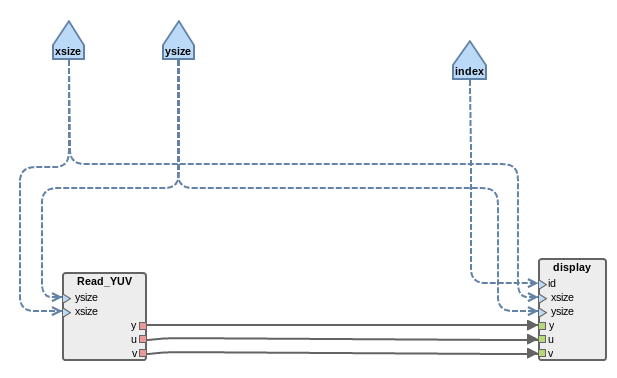
\includegraphics[width=0.99\textwidth]{images/example_preesm_diagram.png}
    \caption{A simple dataflow diagram used by PREESM} \end{center}
\end{figure}

In the experiment \ref{sec:firstexperiment} a baseline application for comparison
with OpenEM was needed. PREESM was selected because it is capable of code
generation for TMS320C6678, introduced in chapter \ref{chapter:c6678}, and its
simple and fast workflow.

\section{PREESM Internal Representations}
\label{sec:dataflow}
PREESM applications are created by combining inputs of two different
internal representations and manually created source code. The two internal
representations are described here: first the PREESM algorithm representation
PiSDF and second the PREESM hardware model.
\subsection{PiSDF}
The PREESM applications are defined using the Parameterized and Interfaced
Synchronous Dataflow Model of Computation (PiSDF)\cite{pelcat2014preesm}.

Dataflow Model of Computation (MoC) is a directed graph where each node
represents a function and the arcs are the only possible paths the data can
traverse in the graph. In the generic Dataflow MoC the number of tokens produced
or consumed by an actor is not known before execution. For example an actor may
have two output paths and it may choose to produce an output token conditionally
to either one (or both) of the paths. In contrast in Synchronous Data Flow MoC
each actor produces and consumes a pre-determined number of tokens.
\cite{lee1987synchronous} A more thorough explanation of Dataflow MoCs can be
found in \cite{lee2015introduction}.

\subsection{The System-Level Architecture Model (S-LAM)}

\section{Development with PREESM}
\label{sec:preesmdev}

\chapter{Performance Simulation Environment}
\label{chapter:pse}
\section{PSE Introduction}
\section{Resource Network Simulation}

Workload construction, measurements and modeling are discussed in detail in the experiment plan.

The OpenEM programming model and runtime system are studied using \textbf{comparison} and \textbf{modeling} as the methods. A workload application is constructed with a simple runtime system (PREESM) and then converted to OpenEM runtime. The two applications are compared under different load conditions.

The OpenEM application is modeled for resource network simulation. The construction of simulation model needs detailed information about the OpenEM runtime system and the workload application. The data from the measurements is used for the timings needed in the simulation model.

To keep the implementation simple all I/O is omitted from the experiment. The omission of I/O is justified by keeping the experiment strictly focused on the computation in stream processing. The effects of an I/O layer to the studied workload are investigated through literature. 
\chapter{Construction}
\label{chapter:construction}
This chapter describes the implementation of the applications studied in the
experiments. The experiments and their results are described in
\ref{chapter:experiments}. First the common idea behind the video filtering
applications is explained and the filters used are described. After that the
PREESM and OpenEM filter applications are introduced and last the PSE model of
the OpenEM filter application is explained. This chapter is focused on the
design and implementation of the applications.

\section{Filter Application}
\label{sec:filterapp}
Edge detection is an important tool in image processing and computer vision.
Many image processing and computer vision algorithms operate on detected edges.
There is a growing interest in the industry to use DSP platforms for edge
detection based algorithms. In this thesis two filters used in Canny edge
detector are implemented as a part of a image processing application for Texas
Instruments TMS320C6678 DSP. In this section an overview of the Canny edge
detector is given. After that Sobel and Gaussian filter which are both used in
Canny edge detectors and are implemented in this thesis are introduced.\\

TODO: improve intro and find sources for claims. wikipedia on edge detection has
about the same stuff as above.\\
TODO: Explain the why the streams are separate and the frames are not processed
by both of the filters.
\subsection{Canny edge detector}
In his 1986 paper John F. Canny \cite{canny1985computational} lays out the
mathematical criteria for successful edge detection and presents an algorithm,
which is suitable for implementation on DSP platforms and achieves decent edge
detection performance. The Canny Edge Detection consists of five steps
represented in the following list.

\begin{enumerate}
\item{Gaussian filtering}
\item{Sobel filtering}
\item{Non-maximum supression}
\item{Double tresholding}
\item{Edge tracking by hysteresis}
\end{enumerate}

The steps 1. and 2. are implemented in the thesis experiment. Gaussian filtering
is discussed in \ref{subsec:gauss} and sobel filtering in \ref{subsec:sobel}.
The rest of the steps are not implemented in this thesis and thus are only
briefly discussed here.

\subsection{Gaussian filter}
\label{subsec:gauss}
\subsection{Sobel filter}
\label{subsec:gauss}
\section{PREESM Filter Application}
\label{sec:preesmapp}
An actor network is constructed in PREESM that represents the video filter
application. The final PiSDF model of the PREESM video filter application is
presented in figure \ref{preesm_actors}. The PREESM filter application is
adapted from the PREESM tutorial at \cite{preesmtut} by adding another
processing path for gaussian filter and making the necessary modifications to
the shared parts of the application.

\begin{figure}[h!] \label{preesm_actors} \begin{center}
    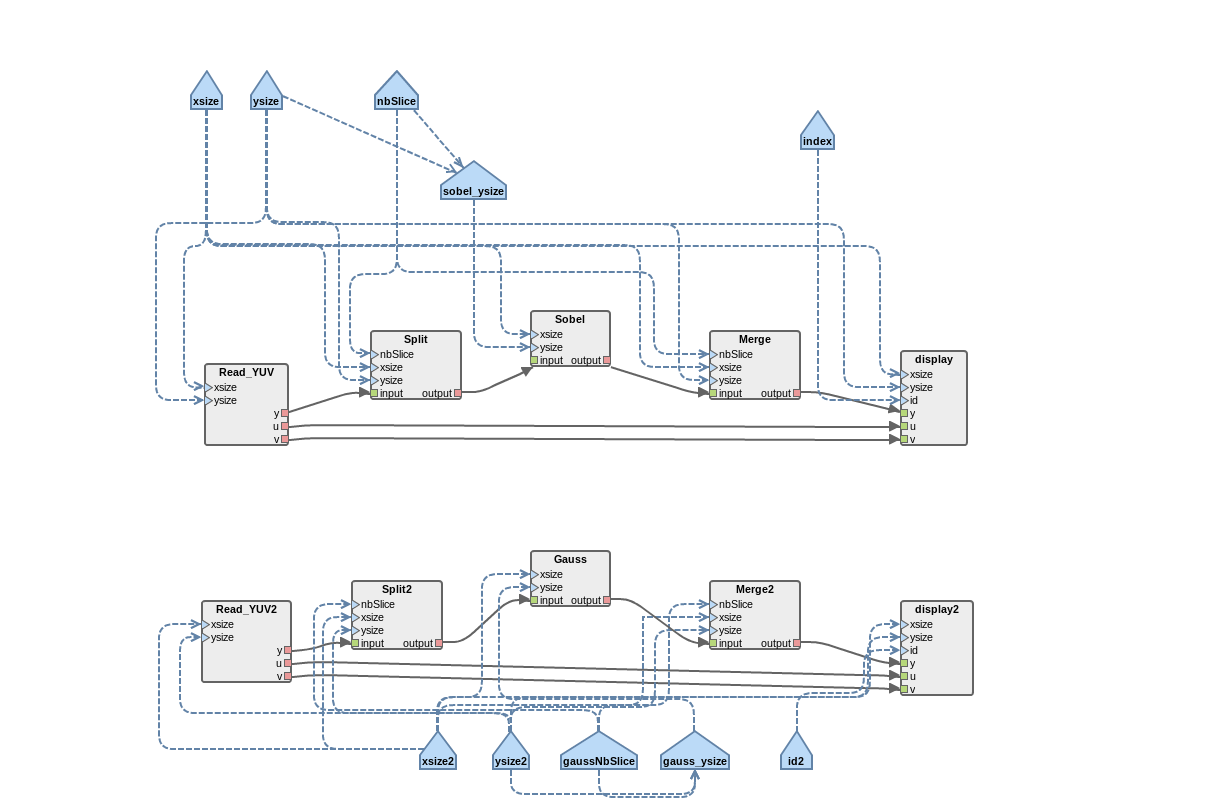
\includegraphics[width=0.99\textwidth]{images/preesm_diagram.png}
    \caption{The PiSDF graph of the PREESM filter application} \end{center}
\end{figure}

To keep the model simple and the program well analyzable both of the processing
paths in the network are independent.

The first actor on both of the processing paths loads the video frames from
memory and passes them to splitting actors. The splitting actor splits the
frames to a suitable number of splices to enable processing of the same video
stream on multiple cores. The filter actor follows the splitting actor. Partial
frames filtered in the filter actor are merged back to whole frames in the merge
actors. The last actors on both of the processing paths are dummy actors.\\

TODO: explain scheduling

\section{OpenEM Filter Application}
The OpenEM implementation of the filter application was heavily influenced by
the PREESM filter application described in \ref{sec:preesmapp}. Specifically the
OpenEM application has to process the frames in similar manner so that only the
scheduling policies between the two programming models should differ. The PREESM
application splits the frames into slices and processes the slices separately
before merging them back into one frame. Similar fork-join mechanism was
implemented in the OpenEM application. Event groups were first planned to be
used as the fork-join mechanism in the filter application but in the final
implementation a different, simpler mechanism was used.

The TI implementation of event groups lacks \texttt{em\_event\_group\_delete}
function which makes it necessary to reuse the existing event groups. The
example applications which are included in the NSN OpenEM distribution
described in \ref{sec:emframework} demonstrate reuse of event groups, but it
was estimated that the programming overhead resulting from the reuse of the
groups would be larger than implementing the fork-join in a simpler manner.

In the final implementation the frames are accumulated simply in a merge buffer
located in shared memory which is referenced through queue context pointers. The
book keeping for frame completion is handled in the same location. The cache
coherency for the book keeping was handled by marking the memory area the merge
buffer resides in as non-cacheable.

\section{PSE Model of OpenEM Filter Application}
\section{Instrumentation}

\chapter [OpenEM Experiments] {Characterizing Open Event Machine Performance
Through Experiments}
\label{chapter:experiments}
The objective of these experiments is to understand the behavior and
performance of the Texas Instruments implementation of Open Event Machine in
realtime stream processing. The objective is achieved by comparing the behavior
of an application implemented using OpenEM to the behavior of a similar
application implemented using a simpler multicore runtime system (PREESM) in the
first part of the experiment. The second part of the experiment is the
construction of a simulation model. The performance predictions from the
simulation model will be compared to the performance of the real world
application. The objective of the comparison is to help better understand the
OpenEM platform.

Both of the experiments are described in a similar manner. First the parameters
and factors of the experiments are explained, second the different measurement
setups are introduced and third the results of the measurements are presented.
The comparison of the PREESM and OpenEM applications is described in the section
\ref{sec:firstexperiment}. The performance of the simulation model is described
in \ref{sec:secondexperiment}.

\section{Comparison of PREESM and OpenEM Filter Applications}
\label{sec:firstexperiment}
In the first experiment the OpenEM and PREESM filter applications were loaded
with similar workloads and their execution was measured. The idea of the first
experiment is to examine the dynamic scheduling capabilities of the OpenEM
scheduler and the overhead of the OpenEM framework in stream processing. The
OpenEM scheduler is hardware accelerated, running on a separate processor in the
TMS320C6678 chip. The scheduling is explained in detail in chapter
\ref{chapter:openem}. To achieve this objective the OpenEM filter application
introduced in chapter \ref{chapter:construction} was measured under different
loads and compared to a similar application implemented using PREESM. The
applications are not comparable in terms of throughput and latency, because the
runtime systems are designed for different purposes. The PREESM application
should be considered a baseline, which demonstrates how a statically scheduled
application behaves under dynamic workload.

The static schedule of the PREESM application was regenerated between every
measurement setup due to the limitations of the code generation in PREESM
framework. The specific limitation was that the parameters of the actor model
were translated in to static memory allocations in the code generator, and
manually changing the generated allocations would have been complicated and
prone to error. As a result the actors are scheduled slightly differently
between each scenario. The schedules differ in the mapping of actors to cores
but not in ordering of the actors. The actor ordering is defined by the
dependencies between the actors and availability of computing resources. To
demonstrate the effect of static scheduling, the estimated actor timings of the
PREESM application were not modified when changing the frame size.

In this experiment the applications are loaded with three different workloads
and measured. In addition the OpenEM application is measured under the same load
but different numbers of available cores. The experiment is explained in the
following subsections. In the first subsection the parameters and factors of the
experiment are introduced. Second the different measurement setups are described
and third the results of the experiment are presented.

\subsection{Parameters and Factors}
Dynamic workload conditions are emulated by repeating the measurements with
different factors. To keep things simple the video streams are not dynamically
switched at runtime. The measurement parameters are presented in the following
listing.

\begin{itemize}
    \item \textbf{Video Frame Size} - The workloads are differentiated by
        changing the frame sizes of the video streams.
    \item \textbf{OpenEM Core Masks} - The OpenEM application is measured
        with different core masks of the Execution Objects.
    \item \textbf{Number of Frames Processed Simultaneously} - The OpenEM
        application processes variable number of frames simultaneously, which
        affects the latency and throughput of the application.
\end{itemize}

The different video frame sizes used are presented in table
\ref{tab:cif_frames}. The frame sizes used are selected from among the Common
Intermediate Format frame sizes. TODO: find a reference for CIF. YUV video
format is used in the applications, but only the Y channel is processed by the
applications. The Y channel in the YUV frame contains $R_{x} * R_{y}$ bytes
where $R$ is the resolution. In the YUV format used the U and V channels have
reduced bitrates of $\frac{1}{4} * R_{x} * R_{y}$ per frame.

\begin{table}
    \begin{center}
        \begin{tabular}{ c c c }
            Name  & X resolution  & Y resolution \\ \hline
            QCIF  & 176           & 144          \\ \hline
            CIF   & 352           & 288          \\ \hline
            4CIF  & 704           & 576          \\ \hline
        \end{tabular}
        \caption{CIF frame sizes}
        \label{tab:cif_frames}
    \end{center}
\end{table}

In the second part of this experiment OpenEM core masks are used to limit the
number of cores available to the filter application. The behavior of OpenEM is
examined under limited resources. The core masks in Texas Instruments
implementation of OpenEM are limited so that only one core mask can be active in
the application as discussed in chapter \ref{chapter:openem}, therefore the core
masks always apply to all execution objects of the application.

\subsection{Measurement Setups}
The filter applications process two video streams simultaneously as described in
chapter \ref{chapter:construction}. One video stream is processed with a sobel
filter and the other is processed with a gaussian filter. The dynamic behavior
of the applications is investigated using different workloads. The workloads
used are presented in the table \ref{tab:preesm_setups}. The purpose of the
different bitrates used for each video stream is to expose the behavior of the
OpenEM scheduler in handling dynamic workloads. The static schedule in the
PREESM application will provide a baseline to reflect the OpenEM performance to,
but again the performance of the applications should not be directly compared
due to the difference in the runtime systems.

In addition to comparing the PREESM and OpenEM applications the OpenEM
application is measured with different core masks to investigate the dynamic
scheduling with different limitations. Both filters of the OpenEM application
are loaded with CIF streams and different numbers of cores are used. The
experiment is run with core masks allowing one to eight cores being used for
processing the streams.

\begin{table}
    \begin{center}
        \begin{tabular}{ c c }
            Sobel Resolution & Gauss Resolution \\ \hline
            CIF              & CIF              \\ \hline
            4CIF             & CIF              \\ \hline
            CIF              & 4CIF             \\ \hline
            QCIF             & QCIF             \\ \hline
        \end{tabular}
        \caption{PREESM and OpenEM measurement setups}
        \label{tab:preesm_setups}
    \end{center}
\end{table}

\subsection{Results}
In this subsection first the results of the measurements of the OpenEM and
PREESM applications are presented and next the results of measuring the OpenEM
application limited with core masks are presented. The latency and throughput of
the OpenEM application measurements are summarized in the table
\ref{tab:oemthrough} and in table \ref{tab:preesmthrough} of the PREESM
application. The summary of latency and throughtput of the OpenEM application
with limited number of cores is presented in table \ref{tab:oemcoremasks}.

The latency of both of the filters is measured from the time the frame is loaded
from the memory to the time the frame is merged after filtering. The throughput
is measured as frames per second processed in total by the application. Since
both of the applications process frames at the same rate from both streams,
there is only one FPS measurement for each of the measurement setups.

The PREESM latencies in the table \ref{tab:preesmthrough} are consistently
smaller than the latencies of the OpenEM application in the table
\ref{tab:oemthrough}. This corresponds to the difference of the block schedule
used in the PREESM application to the dynamic schedule used in the OpenEM
application. The OpenEM schedule is more optimized for throughput which is
readily observed from the difference of the FPS metrics for both applications.
The throughput versus latency balance in the OpenEM application is controlled
through the number of frames processed simultaneously. In this set of
measurements the OpenEM application is configured to process 16 frames
simultaneously to maximize throughput. \\

TODO: Add another set of OpenEM measurements using smaller number of initial
events for better latency.\\

\newcommand{\head}[2]{\multicolumn{1}{>{\centering\arraybackslash}p{#1}}{#2}}
\begin{table}
    \begin{center}
        \begin{tabular}{ c c c c c }
            \head{1.5cm}{Sobel latency} & \head{1.5cm}{Gauss latency} &
            \head{1.5cm}{FPS} & \head{1.5cm}{Sobel frame} &
            \head{1.5cm}{Gauss frame} \\ \hline
            5,41 & 8,78 & 223 & CIF & 4CIF \\ \hline
            4,65 & 3,54 & 334 & 4CIF & CIF \\ \hline
            2,15 & 2,51 & 668 & CIF & CIF \\ \hline
            0,61 & 0,71 & 2004 & QCIF & QCIF \\ \hline
        \end{tabular}
        \caption{PREESM latency and throughput. The the latencies are measured
        in milliseconds.}
        \label{tab:preesmthrough}
    \end{center}
\end{table}

\begin{table}
    \begin{center}
        \begin{tabular}{ c c c c c }
            \head{1.5cm}{Sobel latency} & \head{1.5cm}{Gauss latency} &
            \head{1.5cm}{FPS} & \head{1.5cm}{Sobel frame} &
            \head{1.5cm}{Gauss frame} \\ \hline
            15,82 & 22,85 & 599 & CIF & 4CIF \\ \hline
            4,85 & 3,67 & 895 & 4CIF & CIF \\ \hline
            4,91 & 5,96 & 1955 & CIF & CIF \\ \hline
            1,33 & 1,62 & 7819 & QCIF & QCIF \\ \hline
        \end{tabular}
        \caption{OpenEM latency and throughput. The latencies are measured in
        milliseconds.}
        \label{tab:oemthrough}
    \end{center}
\end{table}

A block schedule could be generated, which would yield a higher throughput by
introducing multiple instances of the actors for each repetition of the
schedule. The successive repetitions of the schedule would be interleaved and
the overhead of synchronizing the cores would be reduced. The current version of
PREESM does not support the described interleaving of the repetitions
\cite{pelcat2014preesm}. TODO: this belongs to discussion / conclusions.

The throughput of the application is determined by how much time the application
spends processing the streams versus the time spent doing something else. For
example the synchronization of all cores before each repetition of the PREESM
schedule consumes a lot of cpu cycles as is readily observed from the figure
\ref{fig:preesmcif}. The portion of the bars marked as busy corresponds to the
cycles spent in the synchronization between the repetitions of the schedule. The
percentage of cycles spent in the synchronization varies from 16\% on Core 7
to 45\% on Core 0. Comparing the core utilization of the PREESM application to
the core utilization of the OpenEM application presented in the figure
\ref{fig:oem8corefunc} the differences in the schedulers start to become apparent.

\begin{figure}
    \centering
    \begin{subfigure}[t]{0.49\textwidth}
        \centering
        \includegraphics[width=0.99\linewidth]{images/preesm_cifcif.eps}
        \caption{PREESM}
        \label{fig:preesmcif}
    \end{subfigure}
    \begin{subfigure}[t]{0.49\textwidth}
        \centering
        \includegraphics[width=0.99\linewidth]{images/openem_cifcif_8cores_func.eps}
        \caption{OpenEM}
        \label{fig:oem8corefunc}
    \end{subfigure}
    \caption{In the PREESM graph the busy portion of the bars correspond to the
        cycles spent synchronizing the cores between the repetitions of the
        block schedule. The overhead corresponds to cycles spent outside the
        measured functions and the busy cycles. In the OpenEM graph the overhead
        corresponds to cycles spent outside the listed functions, which includes
    the communication overhead and the copying of the data between the buffers.}
\end{figure}

One to one comparison of the cpu utilization of the applications is difficult
due to the differences in the runtime systems. The overhead portions in the
figures \ref{fig:preesmcif} and \ref{fig:oem8corefunc} contain all of the data
copying from buffer to buffer outside the measured functions, but they also
contain different amounts of cycles spent in communications between the cores. A
more revealing view at the overhead of the OpenEM runtime is found by looking at
the cycles spent per execution object in the OpenEM application in figure
\ref{fig:oem8coreeo}, where the overhead corresponds to cycles spent outside the
execution objects. The cycles spent outside the execution objects are maximum of
3\% on all cores.

The throughput of both of the applications scales roughly in proportion to each
other across the different workloads in tables \ref{tab:preesmthrough} and
\ref{tab:oemthrough}. However the latencies of the OpenEM application show more
variable behavior. The latencies of both applications are roughly the same in
the case of two CIF streams and are improved roughly by a factor of 3.5 when the
bitrates are decreased in the case of two QCIF streams. The latencies of the
PREESM application grow steadily as the load of the application is increased.
The latencies of the OpenEM application actually improve when the resolution of
the sobel stream is increased to 4CIF and then drastically grow in the heaviest
workload case with sobel resolution of CIF and gauss resolution of 4CIF.

The probable cause of the improvement of the latencies when the workload is made
heavier by increasing the sobel stream resolution is the reduced interleaving of
the processing of the subsequent frames. The reduction in the interleaving is
caused by the read execution object which is only connected to an atomic queue.
When the frame size of the sobel stream is increased the read EO starts limiting
the throughput of the application. Fewer frames are processed in parallel which
decreases the time from reading each individual frame to the completion of that
frame. The formation of the bottleneck can be observed by comparing the core
utilization in the figure \ref{fig:oem8coreeo} to the core utilization in the
figure \ref{fig:oem8coreeosobel4cif} where seven cores need to wait for the read
operations on the Core 2 and the overall overhead is increased. The other cores
do not receive any events from the OpenEM scheduler while waiting. TODO:
discussion/ conclusions

\begin{figure}
    \centering
    \begin{subfigure}[t]{0.49\textwidth}
        \centering
        \includegraphics[width=0.99\linewidth]{images/openem_cifcif_8cores_eo.eps}
        \caption{Sobel CIF, Gauss CIF}
        \label{fig:oem8coreeo}
    \end{subfigure}
    \begin{subfigure}[t]{0.49\textwidth}
        \centering
        \includegraphics[width=0.99\linewidth]{images/openem_sobel4cif_gausscif_eo.eps}
        \caption{Sobel 4CIF, Gauss Cif}
        \label{fig:oem8coreeosobel4cif}
    \end{subfigure}
    \caption{The bottleneck forming due to the atomic read operation can be
    observed by comparing the core utilization when both of the streams are at
    CIF resolution to the case where sobel resolution is increased to 4CIF.}
\end{figure}

When the gauss stream is increased to 4CIF and the sobel stream is kept at CIF
the bottleneck does not form because computing the gaussian filter for the 4CIF
frames is consuming approximately 80\% of the cycles on all cores. In this case
the read EO only consumes approximately 5\% to 13\% of the cycles on all cores.
Compared to the case of two CIF streams, the latencies in this case are
increased by factors of approximately 3 and 4 for sobel and gauss
correspondingly. The resulting core utilization graph is presented in figure
\ref{fig:oem8coreeogauss4cif}.

\begin{figure}[h]
    \begin{center}
        \includegraphics[width=0.49\textwidth]{images/openem_sobelcif_gauss4cif_eo.eps}
        \caption{OpenEM cycles spent per execution object for CIF sobel frames
        and 4CIF gauss frames}
        \label{fig:oem8coreeogauss4cif}
    \end{center}
\end{figure}

\begin{table}
    \begin{center}
        \begin{tabular}{ c c c c }
            \head{1.5cm}{Sobel latency} & \head{1.5cm}{Gauss latency} &
            \head{1.5cm}{FPS} & \head{1.5cm}{Number of cores} \\
            \hline
            57,05 & 57,11 & 263 & 1 \\ \hline
            22,59 & 23,15 & 510 & 2 \\ \hline
            15,09 & 15,84 & 768 & 3 \\ \hline
            10,91 & 11,85 & 1014 & 4 \\ \hline
            8,41 & 9,53 & 1268 & 5 \\ \hline
            7,05 & 8,07 & 1500 & 6 \\ \hline
            5,74 & 6,83 & 1731 & 7 \\ \hline
            4,91 & 5,96 & 1955 & 8 \\ \hline
        \end{tabular}
        \caption{OpenEM measurements with number of cores varied}
        \label{tab:oemcoremasks}
    \end{center}
\end{table}

The second part of this experiment was to limit the number of cores available
for the OpenEM application. The resulting latencies and throughputs are
presented in the table \ref{tab:oemcoremasks}. The increase of the throughput of
the OpenEM application is presented in graph \ref{fig:fpsvcores}. The actual FPS
measured with eight cores is approximately 90\% of the linear growth.

\begin{figure}[h!]
    \begin{center}
        \includegraphics[width=0.7\textwidth]{images/coremask_fps.eps}
        \caption{FPS increase as the function of cores vs. linear growth}
        \label{fig:fpsvcores}
    \end{center}
\end{figure}

\section{Comparison of Simulated OpenEM Performance and Real OpenEM Performance}
\label{sec:secondexperiment}
\subsection{Parameters and Factors}
\subsection{Measurement Setups}
\subsection{Results}


\chapter{Discussion}
\label{chapter:discussion}
\section{Challenges}
\section{Related Work}
\section{Future Work}

\chapter{Conclusions}
\label{chapter:conclusion}
\fixme{re-write the first paragraphs} \\
\fixme{From suitability to performance} \\
\fixme{Answers to the questions set in the problem statement} \\
This thesis set out to analyse the suitability of the Texas Instruments implementation of the Open Event Machine multicore runtime to stream processing. The results suggest that OpenEM runtime is flexible enough to support the implementation of such applications. Further research is required to understand the overall suitability of multicore DSPs for stream processing.

A video stream processing application inspired by Canny edge detector was designed. The design was implemented using two distinct multicore runtimes. The baseline application was implemented using PREESM, which generates statically scheduled multicore applications based on synchronous dataflow graphs. The main system under study of this thesis was the OpenEM implementation of the design. To understand the application behavior both applications were instrumented and their execution was measured. The statically scheduled PREESM application achieved lower latency in most of the conducted measurements but the OpenEM application was shown to be well configurable and able to handle dynamic workloads.

High performance stream processing solutions are in demand in the industry. Exploring the use of DSP for stream processing is interesting because they achieve high ratio of floating point operations to power consumption. As multicore DSPs are not as commonly used for stream processing as for example GPUs, the tools for parallel programming have not converged. Runtime systems such as OpenEM have the potential of becoming the standard tools for parallel programming of DSPs.

% Load the bibliographic references
% ------------------------------------------------------------------
% You can use several .bib files:
% \bibliography{thesis_sources,ietf_sources}
\bibliography{sources}


% Appendices go here
% ------------------------------------------------------------------
% If you do not have appendices, comment out the following lines
\appendix
\chapter{First appendix: OpenEM and PREESM comparison}
\label{chapter:first-appendix}

\begin{figure}[h!]
    \begin{center}
        \includegraphics[width=0.99\textwidth]{images/openem_cifcif_8cores_eo.eps}
        \caption{OpenEM cycles spent per execution object for CIF sobel frames and CIF gauss frames}
%        \label{fig:oem8coreeo}
    \end{center}
\end{figure}

\begin{figure}[h!]
    \begin{center}
        \includegraphics[width=0.99\textwidth]{images/openem_cifcif_8cores_func.eps}
        \caption{OpenEM cycles spent per function for CIF sobel frames and CIF gauss frames}
%        \label{fig:oem8corefunc}
    \end{center}
\end{figure}

\begin{figure}[h!]
    \begin{center}
        \includegraphics[width=0.99\textwidth]{images/openem_sobel4cif_gausscif_eo.eps}
        \caption{OpenEM cycles spent per execution object for 4CIF sobel frames and CIF gauss frames}
%        \label{fig:oem8coreeosobel4cif}
    \end{center}
\end{figure}

\begin{figure}[h!]
    \begin{center}
        \includegraphics[width=0.99\textwidth]{images/openem_sobel4cif_gausscif_func.eps}
        \caption{OpenEM cycles spent per function for 4CIF sobel frames and CIF gauss frames}
        \label{fig:oem8corefuncsobel4cif}
    \end{center}
\end{figure}

\begin{figure}[h!]
    \begin{center}
        \includegraphics[width=0.99\textwidth]{images/openem_sobelcif_gauss4cif_eo.eps}
        \caption{OpenEM cycles spent per execution object for CIF sobel frames and 4CIF gauss frames}
%        \label{fig:oem8coreeogauss4cif}
    \end{center}
\end{figure}

\begin{figure}[h!]
    \begin{center}
        \includegraphics[width=0.99\textwidth]{images/openem_sobelcif_gauss4cif_func.eps}
        \caption{OpenEM cycles spent per function for CIF sobel frames and 4CIF gauss frames}
        \label{fig:oem8corefuncgauss4cif}
    \end{center}
\end{figure}

\begin{figure}[h!]
    \begin{center}
        \includegraphics[width=0.99\textwidth]{images/openem_sobelqcif_gaussqcif_eo.eps}
        \caption{OpenEM cycles spent per execution object for QCIF sobel frames and QCIF gauss frames}
        \label{fig:oem8coreeoqcif}
    \end{center}
\end{figure}

\begin{figure}[h!]
    \begin{center}
        \includegraphics[width=0.99\textwidth]{images/openem_sobelqcif_gaussqcif_func.eps}
        \caption{OpenEM cycles spent per function for CIF sobel frames and 4CIF gauss frames}
        \label{fig:oem8corefuncqcif}
    \end{center}
\end{figure}

\begin{figure}[h!]
    \begin{center}
        \includegraphics[width=0.99\textwidth]{images/preesm_cifcif.eps}
        \caption{PREESM cycles spent per function for CIF sobel frames and CIF gauss frames}
%        \label{fig:preesmcif}
    \end{center}
\end{figure}

\begin{figure}[h!]
    \begin{center}
        \includegraphics[width=0.99\textwidth]{images/preesm_sobel4cif_gausscif.eps}
        \caption{PREESM cycles spent per function for 4CIF sobel frames and CIF gauss frames}
        \label{fig:preesmsobel4cif}
    \end{center}
\end{figure}

\begin{figure}[h!]
    \begin{center}
        \includegraphics[width=0.99\textwidth]{images/preesm_sobelcif_gauss4cif.eps}
        \caption{PREESM cycles spent per function for CIF sobel frames and 4CIF gauss frames}
        \label{fig:preesmgauss4cif}
    \end{center}
\end{figure}

\begin{figure}[h!]
    \begin{center}
        \includegraphics[width=0.99\textwidth]{images/preesm_sobelqcif_gaussqcif.eps}
        \caption{PREESM cycles spent per function for QCIF sobel frames and QCIF gauss frames}
        \label{fig:preesmgauss4cif}
    \end{center}
\end{figure}


\chapter{Second Appendix: OpenEM coremasks}

\begin{figure}[h!]
    \begin{center}
        \includegraphics[width=0.99\textwidth]{images/openem_cifcif_1cores_eo.eps}
        \caption{OpenEM cycles spent per execution object for CIF sobel frames and CIF gauss frames using 1 core.}
        \label{fig:oem1coreeo}
    \end{center}
\end{figure}

\begin{figure}[h!]
    \begin{center}
        \includegraphics[width=0.99\textwidth]{images/openem_cifcif_1cores_func.eps}
        \caption{OpenEM cycles spent per function for CIF sobel frames and CIF gauss frames using 1 core.}
        \label{fig:oem1corefunc}
    \end{center}
\end{figure}


\begin{figure}[h!]
    \begin{center}
        \includegraphics[width=0.99\textwidth]{images/openem_cifcif_2cores_eo.eps}
        \caption{OpenEM cycles spent per execution object for CIF sobel frames and CIF gauss frames using 2 cores.}
        \label{fig:oem2coreeo}
    \end{center}
\end{figure}

\begin{figure}[h!]
    \begin{center}
        \includegraphics[width=0.99\textwidth]{images/openem_cifcif_2cores_func.eps}
        \caption{OpenEM cycles spent per function for CIF sobel frames and CIF gauss frames using 2 cores.}
        \label{fig:oem2corefunc}
    \end{center}
\end{figure}


\begin{figure}[h!]
    \begin{center}
        \includegraphics[width=0.99\textwidth]{images/openem_cifcif_3cores_eo.eps}
        \caption{OpenEM cycles spent per execution object for CIF sobel frames and CIF gauss frames using 3 cores.}
        \label{fig:oem3coreeo}
    \end{center}
\end{figure}

\begin{figure}[h!]
    \begin{center}
        \includegraphics[width=0.99\textwidth]{images/openem_cifcif_3cores_func.eps}
        \caption{OpenEM cycles spent per function for CIF sobel frames and CIF gauss frames using 3 cores.}
        \label{fig:oem3corefunc}
    \end{center}
\end{figure}


\begin{figure}[h!]
    \begin{center}
        \includegraphics[width=0.99\textwidth]{images/openem_cifcif_4cores_eo.eps}
        \caption{OpenEM cycles spent per execution object for CIF sobel frames and CIF gauss frames using 4 cores.}
        \label{fig:oem4coreeo}
    \end{center}
\end{figure}

\begin{figure}[h!]
    \begin{center}
        \includegraphics[width=0.99\textwidth]{images/openem_cifcif_4cores_func.eps}
        \caption{OpenEM cycles spent per function for CIF sobel frames and CIF gauss frames using 4 cores.}
        \label{fig:oem3corefunc}
    \end{center}
\end{figure}


\begin{figure}[h!]
    \begin{center}
        \includegraphics[width=0.99\textwidth]{images/openem_cifcif_5cores_eo.eps}
        \caption{OpenEM cycles spent per execution object for CIF sobel frames and CIF gauss frames using 5 cores.}
        \label{fig:oem5coreeo}
    \end{center}
\end{figure}

\begin{figure}[h!]
    \begin{center}
        \includegraphics[width=0.99\textwidth]{images/openem_cifcif_5cores_func.eps}
        \caption{OpenEM cycles spent per function for CIF sobel frames and CIF gauss frames using 5 cores.}
        \label{fig:oem5corefunc}
    \end{center}
\end{figure}


\begin{figure}[h!]
    \begin{center}
        \includegraphics[width=0.99\textwidth]{images/openem_cifcif_6cores_eo.eps}
        \caption{OpenEM cycles spent per execution object for CIF sobel frames and CIF gauss frames using 6 cores.}
        \label{fig:oem6coreeo}
    \end{center}
\end{figure}

\begin{figure}[h!]
    \begin{center}
        \includegraphics[width=0.99\textwidth]{images/openem_cifcif_6cores_func.eps}
        \caption{OpenEM cycles spent per function for CIF sobel frames and CIF gauss frames using 6 cores.}
        \label{fig:oem2corefunc}
    \end{center}
\end{figure}

\begin{figure}[h!]
    \begin{center}
        \includegraphics[width=0.99\textwidth]{images/openem_cifcif_7cores_eo.eps}
        \caption{OpenEM cycles spent per execution object for CIF sobel frames and CIF gauss frames using 7 cores.}
        \label{fig:oem7coreeo}
    \end{center}
\end{figure}

\begin{figure}[h!]
    \begin{center}
        \includegraphics[width=0.99\textwidth]{images/openem_cifcif_7cores_func.eps}
        \caption{OpenEM cycles spent per function for CIF sobel frames and CIF gauss frames using 7 cores.}
        \label{fig:oem7corefunc}
    \end{center}
\end{figure}

\begin{figure}[h!]
    \begin{center}
        \includegraphics[width=0.99\textwidth]{images/openem_cifcif_8cores_eo.eps}
        \caption{OpenEM cycles spent per execution object for CIF sobel frames and CIF gauss frames using 8 cores.}
        \label{fig:oem8coreeo2}
    \end{center}
\end{figure}

\begin{figure}[h!]
    \begin{center}
        \includegraphics[width=0.99\textwidth]{images/openem_cifcif_8cores_func.eps}
        \caption{OpenEM cycles spent per function for CIF sobel frames and CIF gauss frames using 8 cores.}
        \label{fig:oem8corefunc2}
    \end{center}
\end{figure}

\begin{figure}[h!]
    \begin{center}
        \includegraphics[width=0.99\textwidth]{images/coremask_fps.eps}
        \caption{FPS increase as the function of cores vs. linear growth}
%        \label{fig:fpsvcores}
    \end{center}
\end{figure}

\begin{figure}[h!]
    \begin{center}
        \includegraphics[width=0.99\textwidth]{images/coremask_latencies.eps}
        \caption{Latency decrease as the function of cores}
        \label{fig:latencyvcores}
    \end{center}
\end{figure}


% End of document!
% ------------------------------------------------------------------
% The LastPage package automatically places a label on the last page.
% That works better than placing a label here manually, because the
% label might not go to the actual last page, if LaTeX needs to place
% floats (that is, figures, tables, and such) to the end of the 
% document.
\end{document}
